% !TEX root = ../../../main.tex
% 所属：第一部分：单变量分析学 / 第5章：级数理论
% 节：5.4 级数的绝对收敛与条件收敛
% 正文按原文件顺序保存；由 ../chapter5.tex 调用。
\section{级数的绝对收敛与条件收敛}
\begin{definition}
	对级数 $\sum a_n$，若级数 $\sum |a_n|$ 收敛，则称级数 $\sum a_n$ \text{绝对收敛}。
	
	由不等式
	\[
	|a_{n+1} + a_{n+2} + \dots + a_{n+p}| \le |a_{n+1}| + |a_{n+2}| + \dots + |a_{n+p}| < \varepsilon
	\]
	可知：\text{绝对收敛的级数必收敛}。
	若级数 $\sum a_n$ 收敛，但不绝对收敛，则称级数 $\sum a_n$ 条件收敛。
\end{definition}

\begin{example}
	讨论级数 $\displaystyle \sum_{n=1}^{\infty} \frac{x^n}{n^p}$ 的敛散性
	
\end{example}
\begin{solution}
	对其绝对值级数
	\[
	\sum_{n=1}^{\infty} \left| \frac{x^n}{n^p} \right| = \sum_{n=1}^{\infty} \frac{|x|^n}{n^p}
	\]
	应用 Cauchy 判别法：
	\[
	\lim_{n \to \infty} \sqrt[n]{\frac{|x|^n}{n^p}} = |x|
	\]
	
	\begin{itemize}
		\item 若 $|x| < 1$，对任意 $p \in \mathbb{R}$，级数绝对收敛。
		\item 若 $|x| > 1$，对任意 $p \in \mathbb{R}$，级数发散。
	\end{itemize}
	
	接下来讨论边界情况：
	
	\begin{itemize}
		\item \text{当 $x=1$ 时}：级数为 $\displaystyle \sum_{n=1}^{\infty} \frac{1}{n^p}$，即 $p$-级数：
		\begin{itemize}
			\item $p > 1$：级数绝对收敛；
			\item $p \le 1$：级数发散。
		\end{itemize}
		
		\item \text{当 $x=-1$ 时}：级数为 $\displaystyle \sum_{n=1}^{\infty} \frac{(-1)^n}{n^p}$：
		\begin{itemize}
			\item $p > 1$：级数绝对收敛；
			\item $0 < p \le 1$：级数条件收敛（由 Leibniz 判别法）；
			\item $p \le 0$：级数发散（通项不趋于0）。
		\end{itemize}
	\end{itemize}
	
\end{solution}
\begin{definition}
	将级数 $\sum x_n$ 求和中的数列 $\{x_n\}$ 的次序重新排列，但不新增也不遗漏。
	
	设所得的数列为 $\{x'_n\}$，对应的级数为 $\sum x'_n$，称之为 $\sum x_n$ 的 \text{更序级数}。
	$\sum x_n$ 也为 $\sum x'_n$ 的更序级数，称这一过程为 \text{级数的重排}。
\end{definition}
\begin{example}
	考虑级数
	\[
	\sum_{n=1}^{\infty} \frac{(-1)^{n+1}}{n} = \ln 2
	\]
	的重排：
	\[
	1 - \frac{1}{2} - \frac{1}{4} + \frac{1}{3} - \frac{1}{6} - \frac{1}{8} + \dots = \sum x'_n
	\]
\end{example}

\begin{solution}
	设原级数的部分和为 $S_n = \sum\limits_{k=1}^{n} \dfrac{(-1)^{k+1}}{k}$。
	重排级数的部分和
	\[
	\begin{aligned}
		S'_{3n} &= 1 - \frac{1}{2} - \frac{1}{4} + \dots + \left( \frac{1}{2n-1} - \frac{1}{4n-2} - \frac{1}{4n} \right) \\
		&= \sum_{k=1}^{n} \left( \frac{1}{4k-2} - \frac{1}{4k} \right) \\
		&= \frac{1}{2} \sum_{k=1}^{n} \left( \frac{1}{2k-1} - \frac{1}{2k} \right) \\
		&= \frac{1}{2} \left( 1 - \frac{1}{2} + \frac{1}{3} - \frac{1}{4} + \dots \right) = \frac{1}{2} S_{2n} \to \frac{1}{2} \ln 2
	\end{aligned}
	\]
	而
	\[
	S'_{3n-1} = S'_{3n} + \frac{1}{4n} \to \frac{1}{2} \ln 2
	\]
	\[
	S'_{3n-2} = S'_{3n} + \frac{1}{4n} + \frac{1}{4n-2} \to \frac{1}{2} \ln 2
	\]
	故更序级数收敛于 $\dfrac{1}{2} \ln 2$。
\end{solution}

\begin{definition}
	设 $\sum\limits_{n=1}^{\infty} x_n$ 是任意项级数，令
	\[
	x_n^+ = \frac{|x_n| + x_n}{2} =
	\begin{cases}
		x_n, & x_n > 0 \\
		0, & x_n \le 0
	\end{cases}
	\quad n=1,2,\dots
	\]
	\[
	x_n^- = \frac{|x_n| - x_n}{2} =
	\begin{cases}
		-x_n, & x_n < 0 \\
		0, & x_n \ge 0
	\end{cases}
	\quad n=1,2,\dots
	\]
	则
	\[
	x_n = x_n^+ - x_n^-, \quad |x_n| = x_n^+ + x_n^- \quad n=1,2,\dots
	\]
	且 $\sum x_n^+$ 与 $\sum x_n^-$ 都是正项级数。
\end{definition}
\begin{proposition}\label{ 绝对收敛}
	\begin{itemize}
		\item 若 $\sum x_n$ 绝对收敛，则 $\sum x_n^+$ 与 $\sum x_n^-$ 都收敛；
		\item 若 $\sum x_n$ 条件收敛，则 $\sum x_n^+$ 与 $\sum x_n^-$ 都发散到 $+\infty$。
	\end{itemize}

\end{proposition}
\begin{proof}
	先设 $\sum x_n$ 绝对收敛。由
	\[
	0 \le x_n^+ \le |x_n|, \quad 0 \le x_n^- \le |x_n|, \quad n=1,2,\dots
	\]
	根据比较判别法，由 $\sum |x_n|$ 收敛，即得 $\sum x_n^+$ 与 $\sum x_n^-$ 收敛。
	
	现设 $\sum x_n$ 条件收敛。若 $\sum x_n^+$ 收敛，则
	\[
	\sum x_n^- = \sum x_n^+ - \sum x_n
	\]
	可知 $\sum x_n^-$ 也收敛。于是
	\[
	\sum |x_n| = \sum x_n^+ + \sum x_n^-
	\]
	收敛，与 $\sum x_n$ 条件收敛矛盾。故 $\sum x_n^+$ 发散。同理可证 $\sum x_n^-$ 发散。
\end{proof}

\begin{theorem}
	（绝对收敛级数的重排不变性）若级数 $\sum x_n$ 绝对收敛，则其任意更序级数 $\sum x'_n$ 也绝对收敛，且收敛于相同的极限。
	或者说，绝对收敛级数满足加法交换律。
\end{theorem}
\begin{proof}
	先考虑 $\sum x_n$ 为正项级数的情况，设 $\sum x'_n$ 为其更序级数。
	记更序级数的部分和为
	\[
	0 \le S'_k = x'_1 + x'_2 + \dots + x'_k
	\]
	设 $x'_1, x'_2, \dots, x'_k$ 对应原数列 $\{x_n\}$ 中的项为 $x_{n_1}, x_{n_2}, \dots, x_{n_k}$，取
	\[
	m = \max\{n_1, n_2, \dots, n_k\}
	\]
	则有
	\[
	0 \le S'_k \le x_1 + x_2 + \dots + x_m \le \sum_{n=1}^{\infty} x_n
	\]
	故更序级数 $\sum x'_n$ 收敛，且 $\sum x'_n \le \sum x_n$。
	同时，$\sum x_n$ 也是 $\sum x'_n$ 的更序级数，同理有 $\sum x_n \le \sum x'_n$。
	因此
	\[
	\sum_{n=1}^{\infty} x_n = \sum_{n=1}^{\infty} x'_n
	\]
	
	对任意项级数 $\sum x_n$，设 $\sum x'_n$ 为其更序级数。
	由 $\sum x_n$ 绝对收敛，知正项级数 $\sum x_n^+$ 与 $\sum x_n^-$ 都收敛。
	根据正项级数的重排不变性，它们的更序级数 $\sum (x'_n)^+$ 与 $\sum (x'_n)^-$ 也收敛，且收敛值与原级数相同。
	
	于是
	\[
	\sum_{n=1}^{\infty} x'_n = \sum_{n=1}^{\infty} (x'_n)^+ - \sum_{n=1}^{\infty} (x'_n)^- = \sum_{n=1}^{\infty} x_n^+ - \sum_{n=1}^{\infty} x_n^- = \sum_{n=1}^{\infty} x_n
	\]
	且
	\[
	\sum_{n=1}^{\infty} |x'_n| = \sum_{n=1}^{\infty} (x'_n)^+ + \sum_{n=1}^{\infty} (x'_n)^- = \sum_{n=1}^{\infty} |x_n|
	\]
	因此，更序级数 $\sum x'_n$ 也绝对收敛，且和与原级数相同。
	
\end{proof}
 
\begin{theorem}
	（Riemann 重排定理）
	若级数 $\sum x_n$ 条件收敛，则对任意 $a \in \mathbb{R}^*$，存在 $\sum x_n$ 的更序级数 $\sum x'_n$，使得
	\[
	\sum_{n=1}^{\infty} x'_n = a
	\]
\end{theorem}
\begin{proof}
	先考虑 $a \in \mathbb{R}$ 的情况。
	由 $\sum x_n$ 条件收敛，根据\ref{ 绝对收敛}，知 $\sum x_n^+$ 与 $\sum x_n^-$ 都发散到 $+\infty$。
	
	因此，存在正整数 $N_1 \ge 1$，使得
	\[
	x_1^+ + x_2^+ + \dots + x_{N_1-1}^+ < a \quad \text{但} \quad x_1^+ + x_2^+ + \dots + x_{N_1}^+ > a
	\]
	又由 $\sum x_n^- \to +\infty$，存在正整数 $N_2 \ge 1$，使得
	\[
	x_1^+ + \dots + x_{N_1}^+ - x_1^- - \dots - x_{N_2-1}^- > a
	\]
	但
	\[
	x_1^+ + \dots + x_{N_1}^+ - x_1^- - \dots - x_{N_2}^- < a
	\]
	接着，存在正整数 $N_3 \ge N_1$，使得
	\[
	x_1^+ + \dots + x_{N_1}^+ - x_1^- - \dots - x_{N_2}^- + x_{N_1+1}^+ + \dots + x_{N_3-1}^+ < a
	\]
	但
	\[
	x_1^+ + \dots + x_{N_1}^+ - x_1^- - \dots - x_{N_2}^- + x_{N_1+1}^+ + \dots + x_{N_3}^+ > a
	\]
	
	不断重复这个过程，我们得到 $\sum x_n$ 的一个更序级数 $\sum x'_n$，其部分和 $S'_k$ 始终处于 $a$ 的一个邻域中，即存在 $k$，使得
	\[
	a - x_{n_k}^- < S'_k < a + x_{n_k}^+
	\]
	由于原级数收敛，故 $\lim\limits_{n \to \infty} x_n = 0$，从而 $x_{n_k}^+ \to 0$ 且 $x_{n_k}^- \to 0$，因此
	\[
	\lim_{k \to \infty} S'_k = a
	\]
	即 $\sum\limits_{n=1}^{\infty} x'_n = a$。
	
	对 $a = +\infty$ 的情况：
	存在正整数 $N_1 \ge 1$，使得
	\[
	x_1^+ + x_2^+ + \dots + x_{N_1}^+ > 1
	\]
	取 $x_1^-$，再存在正整数 $N_2 \ge N_1$，使得
	\[
	x_1^+ + \dots + x_{N_1}^+ - x_1^- + x_{N_1+1}^+ + \dots + x_{N_2}^+ > 2
	\]
	重复此过程，取出 $N_1, N_2, \dots, N_k, \dots$ 和 $x_1^-, x_2^-, \dots, x_{k-1}^-, \dots$，得到更序级数 $\sum x'_n$，使得对任意 $k$，有
	\[
	x_1^+ + \dots + x_{N_1}^+ - x_1^- + \dots + x_{N_{k-1}+1}^+ + \dots + x_{N_k}^+ > k
	\]
	故 $\sum\limits_{n=1}^{\infty} x'_n = +\infty$。
	
	$a = -\infty$ 时的证明完全类似。
	
\end{proof}



下面我们考虑级数的乘积。对级数 $\sum a_n$ 与 $\sum b_n$，我们考虑它们所有可能的乘积项 $a_i b_j$，这些项可以排列成如下的无穷矩阵：
\[
\begin{array}{ccccc}
	a_1 b_1 & a_1 b_2 & \cdots & a_1 b_m & \cdots \\
	a_2 b_1 & a_2 b_2 & \cdots & a_2 b_m & \cdots \\
	\vdots & \vdots & \ddots & \vdots & \\
	a_n b_1 & a_n b_2 & \cdots & a_n b_m & \cdots \\
	\vdots & \vdots & & \vdots &
\end{array}
\]

我们的一种做法是：
\begin{enumerate}
	\item 先取第一行的有限项相加；
	\item 再取第二行的有限项相加；
	\item $\dots$
	\item 再取第 $k$ 行的有限项相加；
\end{enumerate}
接下来，回到第一行，重复这一过程。

从而，依赖于项的选取与排列，乘积 $(\sum a_n)(\sum b_n)$ 会有无限多种做法。下面介绍两种常用的。

1.对角线排列
\begin{center}
	\centering
	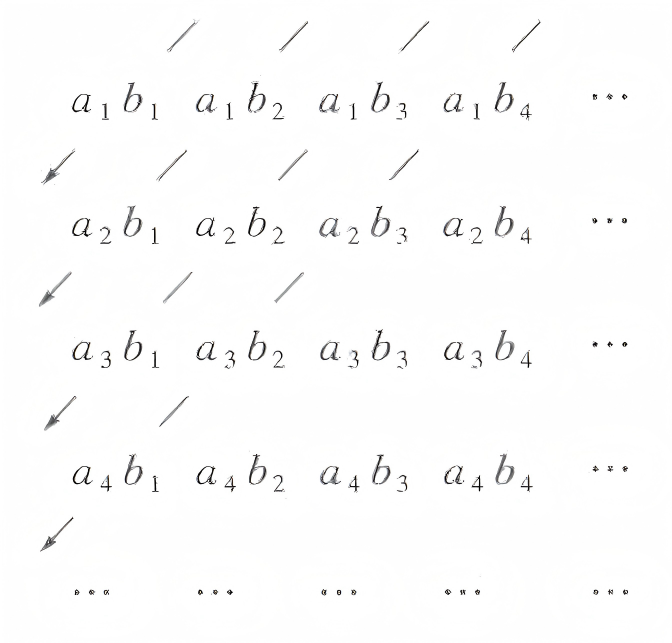
\includegraphics[width=0.4\linewidth]{figure/cauchy(1)}
\end{center}


\[
\begin{aligned}
	c_1 &= a_1 b_1 \\
	c_2 &= a_2 b_1 + a_1 b_2 \\
	&\vdots \\
	c_n &= \sum_{k=1}^n a_k b_{n+1-k}
\end{aligned}
\]
称之为 Cauchy 乘积

2.  正方形排列
\begin{center}
	\centering
	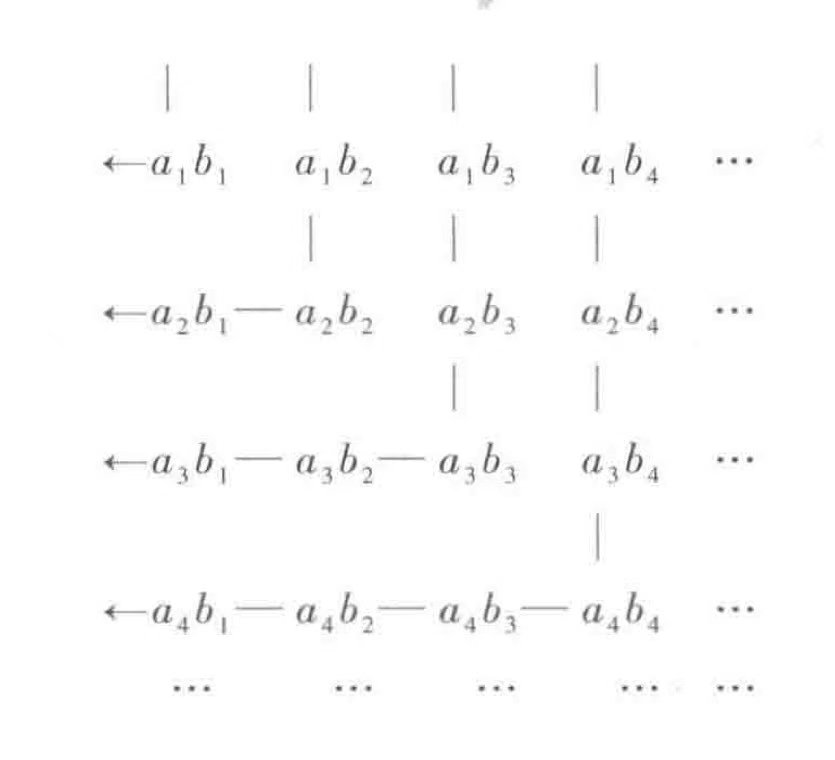
\includegraphics[width=0.4\linewidth]{figure/cubve}
\end{center}


\[
\begin{aligned}
	d_1 &= a_1 b_1 \\
	d_2 &= a_2 b_1 + a_2 b_2 + a_1 b_2 \\
	&\vdots \\
	d_n &= \sum_{k=1}^{n-1} a_n b_k + \sum_{k=1}^{n-1} a_k b_n + a_n b_n
\end{aligned}
\]
其部分和满足：
\[
\sum_{k=1}^n d_k = (a_1 + a_2 + \dots + a_n)(b_1 + b_2 + \dots + b_n)
\]

若级数 $\sum a_n$ 与 $\sum b_n$ 都收敛，则正方形排列的乘积级数 $\sum d_n$ 收敛。设 $\sum a_n = S$，$\sum b_n = T$，则 $\sum d_n = ST$。

但对于 Cauchy 乘积 $\sum c_n$，有可能发散。例如，级数 $\displaystyle \sum_{n=1}^{\infty} \frac{(-1)^{n+1}}{\sqrt{n}}$ 与自身的 Cauchy 乘积发散，而正方形排列的乘积级数收敛。
\begin{proposition}
	（绝对收敛级数的乘积定理）若级数 $\sum a_n$ 与 $\sum b_n$ 都绝对收敛，则将所有乘积项 $a_i b_j$（$i=1,2,\dots; j=1,2,\dots$）按任意方式排列求和而成的级数也绝对收敛，且其和等于
	\[
	\left( \sum_{n=1}^{\infty} a_n \right) \left( \sum_{n=1}^{\infty} b_n \right)
	\]
\end{proposition}
\begin{proof}
	设 $a_{i_k} b_{j_k}$（$k=1,2,\dots$）是所有 $a_i b_j$（$i=1,2,\dots; j=1,2,\dots$）的任意一种排列。对任意正整数 $n$，取
	\[
	N = \max_{1 \le k \le n} \{i_k, j_k\}
	\]
	则
	\[
	\sum_{k=1}^n |a_{i_k} b_{j_k}| \le \sum_{i=1}^N |a_i| \cdot \sum_{i=1}^N |b_i| \le \sum_{n=1}^{\infty} |a_n| \cdot \sum_{n=1}^{\infty} |b_n|
	\]
	因此，级数 $\sum a_{i_k} b_{j_k}$ 绝对收敛。根据绝对收敛级数的重排不变性，其任意更序级数也收敛，且和不变。
	
	设 $\sum d_n$ 是正方形排列下的乘积级数，则 $\sum d_n$ 是 $\sum a_{i_k} b_{j_k}$ 重排后得到的级数。于是
	\[
	\sum_{k=1}^{\infty} a_{i_k} b_{j_k} = \sum_{n=1}^{\infty} d_n = \left( \sum_{n=1}^{\infty} a_n \right) \left( \sum_{n=1}^{\infty} b_n \right)
	\]
\end{proof}
